\section{Die Navier-Stokes-Gleichungen}

\subsection{Todo}

\begin{itemize}
\item
	Erklären, was genau die Navier-Stokes-Gleichungen beschreiben (verhalten
	von Geschwindigkeit des Fluids in einem Gitter)
\item
	Begriff Fluid besser einführen
\item
	Druck genauer erklären (darauf hinweisen, dass es auf den Gradient des
	Drucks ankommt). Grade in Verbindung mit der Helmholtz-Lösung
	weiter unten ist es interessant
\item
	Erklärung mit Partikelsystem und substanzieller Ableitung besser machen.
\end{itemize}

\subsection{Fluide}

Die Gleichungen, die im folgenden beschrieben werden, gelten nicht nur für Gase
wie Luft, sondern auch für Flüssigkeiten wie Wasser. Deshalb wird im Folgenden
der Begriff \PimiddyBegriff{Fluid} verwendet, der beide Zustände zusammenfasst.
Physikalisch gesehen sind Fluide Substanzen, die einer beliebig langsamen
Scherung keinen Widerstand entgegensetzen. Dieses Konzept ist allerdings in
dieser Arbeit nicht von Bedeutung.

Das Volumen von Fluiden ist im Allgemeinen nicht konstant, es wird durch
Veränderung von Druck und Dichte beeinflusst. Dies geschieht z.B. beim
Übertreten der Schallmauer (im Medium Luft) oder bei der Ausbreitung von Tönen
unter Wasser. Bei der Modellierung unterscheidet man allerdings zwischen
\PimiddyBegriff{komprimierbaren} und
\PimiddyBegriff{unkomprimierbaren} Fluiden, je nachdem, ob die Veränderung
des Volumens eine Rolle für die Simulation spielt.

Wir betrachten hier nur \emph{inkompressible} Fluide. Dies stellt kein Problem dar, da
wir nur vergleichsweise kleine Geschwindigkeiten modellieren. Das Modell wird
dadurch allerdings wesentlich vereinfacht.

Zudem haben Fluide im allgemeinen keine konstante \emph{Dichte}. Zur weiteren
Vereinfachung wird hier allerdings von einer konstanten Dichte ausgegangen.

\subsection{Einführung}

Die \PimiddyBegriff{Navier-Stokes-Gleichungen}, benannt nach den Mathematikern
\PimiddyName{Claude-Louis Navier} und \PimiddyName{George Gabriel Stokes},
beschreiben die Bewegung von Fluiden. Die Gleichungen können auf verschiedene
Arten angegeben werden, je nachdem, wie die Fluide modelliert werden. Wir
verwenden hier folgende Form, in der unter anderem die Dichte als konstant
angenommen wird:

\begin{align}
\label{navier_stokes_momentum_equation}
\frac{
	\partial
	\vec{u}
}
{
	\partial t
} +
\vec{u} \PimiddyDiv \vec{u}
& =
\vec{g} +
\nu \PimiddyLaplace \vec{u} -
\frac{
	1
}
{
	\rho
}
\PimiddyGrad p
\\
\label{navier_stokes_incompressibility_condition}
\PimiddyDiv \vec{u} & = 0
\end{align}

\autoref{navier_stokes_momentum_equation} beschreibt eine Differentialgleichung,
die wegen des Terms $\vec{u} \PimiddyDiv \vec{u}$ nichtlinear ist.

Die Gleichungen beschreiben ein Vektorfeld $\vec{u} \colon \PimiddyReell^3 \to
\PimiddyReell^3$, das die \emph{Geschwindigkeit} des Fluids an jedem Punkt im
Raum angibt. Die Gleichungen können genauso gut im zweidimensionalen Raum
betrachtet werden, was im Folgenden auch zur Veranschaulichung getan wird.

\begin{itemize}
\item
	Die Konstante $\rho$ gibt die \emph{Dichte} des Fluids an. Für Wasser beträgt
	sie etwa $700 \frac{kg}{m^3}$, für Wasser etwa $1.3 \frac{kg}{m^3}$.
\item
	Der \emph{Druck} innerhalb des Fluids wird durch das Skalarfeld $p \colon
	\PimiddyReell^3 \to \PimiddyReell$ repräsentiert und spielt bei den späteren
	Berechnungen eine große Rolle.
\item
	Äußere Kräfte wie die Schwerkraft werden im Vektorfeld $\vec{g} \colon
	\PimiddyReell^3 \to \PimiddyReell^3$ zusammengefasst.
\item
	Schließlich unterscheiden sich Fluide in ihrer \PimiddyBegriff{Viskosität} oder
	\PimiddyQuotes{Zähflüssigkeit}, die in der Gleichung mit $\nu$ bezeichnet ist.
	Dickflüssige Fluide wie Honig haben ein hohes $\nu$, dünnflüssige wie Luft ein
	niedriges $\nu$.
\end{itemize}

Gleichung \eqref{navier_stokes_momentum_equation} wird
\PimiddyBegriff{Impulsgleichung} genannt, Gleichung
\eqref{navier_stokes_incompressibility_condition} nennt man
\PimiddyBegriff{Unkomprimierbarkeitsbedingung}. Der Name und die Bedeutung der
Gleichungen werden im Folgenden näher erläutert.

Die Navier-Stokes-Gleichungen komplett zu erläutern geht über den Rahmen dieser
Arbeit weit hinaus, daher soll vor allem ein intuitives Verständnis der
einzelnen Bestandteile gegeben werden. Außerdem soll eine Beziehung zur
klassischen Mechanik hergestellt werden, da die Gleichungen starke Parallelen
hierzu aufweisen.

\subsection{Die Impulsgleichung}

\subsubsection{Lagrange und Euler}

Um Fluide zu modellieren, gibt es zwei Betrachtungsweisen. Die
\PimiddyBegriff{Euler'sche-Betrachtungsweise} und die
\PimiddyBegriff{Lagrange'sche-Betrachtungsweise}.

Bei der \emph{Lagrange'schen-Betrachtungsweise} modellieren wir das Fluid als System
von mikroskopisch kleinen \emph{Partikeln} (man modelliert sozusagen die
Moleküle des Fluids einzeln). Jedes Partikel hat ein Volumen $V$, eine
Masse $m$, eine Position $\vec{x}$ und eine Geschwindigkeit $\vec{u}$. In jedem
Simulationsschritt berechnet man die Kräfte, die auf die Partikel wirken, und
berechnet die resultierende Beschelunigung mit der Newton'schen Formel:

\begin{align*}
m \cdot \vec{a} &= \vec{F} \\
m \cdot \frac{\partial \vec{u}}{\partial t} &= \vec{F}
\end{align*}

Diese Vorgehensweise ist intuitiv und einfach umzusetzen, aber mathematisch
schwer zu analysieren. Beispielsweise kann man die Frage \PimiddyQuotes{Welche
Geschwindigkeit hat das Fluid an Position $\vec{x}$?} nicht sofort
beantworten.

Bei der \emph{Euler'schen-Betrachtungsweise} hingegen hält man jeweils einen Punkt im
Raum fest und analysiert das Strömungsverhalten (Geschwindigkeit, Temperatur)
durch diesen Punkt. Diese Art der Modellierung ist weniger intuitiv, lässt sich
mit Hilfe von Vektorfeldern und Skalarfeldern aber sehr gut mathematisch erfassen.

\subsubsection{Die substantielle Ableitung}

\begin{figure}[ht]
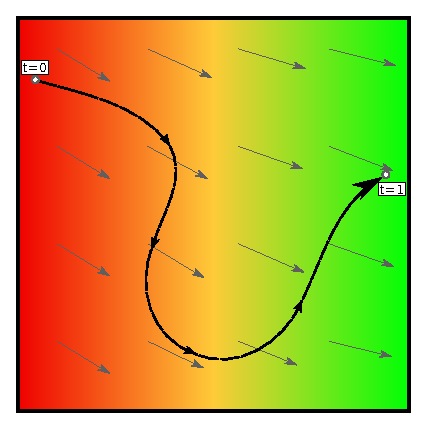
\includegraphics[width=6cm]{images/swimmer_in_water}
\caption{Die Bahn des Schwimmers im Wasser. Die Temperatur des Fluids ist hier durch Farben kodiert. Rot bedeutet warmes Wasser, blau bedeutet kaltes Wasser. Nicht dargestellt ist die Veränderung der Wassertemperatur über die Zeit und die Fließrichtung des Wassers. Die Geschwindigkeit des Gewässers wird fürs erste außer Acht gelassen.}
\end{figure}

Sowohl die Euler'sche- als auch die Lagrang'sche Betrachtungsweise spiegeln sich
in den Navier-Stokes-Gleichungen wider. Sie bilden eine Entsprechung der
klassischen Gleichung $\vec{F} = m \cdot \vec{a}$ mit dem Unterschied, dass
keine Kraft auf einen einzelnen Körper berechnet wird, sondern auf ein
\PimiddyQuotes{Kontinuum}.

Was die beiden Betrachtungsweisen verbindet, ist die
\PimiddyBegriff{substantielle Ableitung}. Zur Herleitung dieser Ableitungsform
betrachten wir zunächst eine beliebige Größe $q(\vec{x},t)$. Dies kann eine
skalare Größe wie z.B. die Temperatur eines Gewässers sein oder eine Vektorgröße
wie die Farbe des Wassers an einem Punkt. Sie ist eine Lagrange'sche Größe, ist
also in jedem Punkt $\vec{x}$ und in jedem Zeitpunkt $t$ gegeben.

Zudem betrachten wir ein Partikel mit einer Bewegungsbahn durch das Fluid (z.B.
einen Schwimmer im Wasser). Seine Position zum Zeitpunkt $t$ sei gegeben durch
$\vec{p}(t)$. Dies entspricht einer Euler'schen Größe.

Setzen wir beide Größen zusammen, erhalten wir beispielsweise die Temperatur des
Wassers auf der Bahn, die der Schwimmer im Wasser verfolgt:

\begin{equation}
\PimiddyFormelText{Temperatur}(t) = q(\vec{p}(t),t)
\end{equation}

Wollen wir wissen, wie sich die Temperatur des Schwimmers im Lauf der Zeit
verändert, bilden wir die (totale) Ableitung dieser zusammengesetzten Größe:

\begin{equation}
\frac{
	\partial \PimiddyFormelText{Temperatur}(t)
}
{
	\partial t
}
=
\frac{
	\partial q
}
{
	\partial t
}
+
\PimiddyGrad q \cdot
\frac{
	\partial \vec{p}}
{
	\partial t
}
\end{equation}

Die Summe auf der rechten Seite besteht aus zwei Teilen. Der erste Term,
$\frac{\partial q}{\partial t}$, gibt an, wie sich das Fluid unabhängig von
der Position verändert. Bezogen auf den Schwimmer gibt dieser Term an, wie
sich die Temperatur des Gewässers über den Tag verteilt verändert. Der
zweite Term ergänzt die Temperaturveränderungen, die durch die Bahn des
Schwimmers verursacht werden.

Statt eines beliebigen Pfades durch das Fluid nimmt man zur Definition der
substantiellen Ableitung nun das Geschwindigkeitsfeld des Fluids zur Hilfe:

\begin{equation}
\frac{
	Dq}
{
	Dt
} :=
\frac{
	\partial q
}
{
	\partial t
}
+
\PimiddyGrad q \cdot
\vec{u}
\end{equation}

Man geht also von einem Partikel aus, was sich im Fluid \PimiddyQuotes{treiben}
lässt, und misst die Veränderung der Größe $q$ auf seiner Bahn. Analog ist die
substantielle Ableitung für Vektorgrößen definiert:

\begin{equation}
\frac{
	D\vec{q}}
{
	Dt
} :=
\frac{
	\partial q
}
{
	\partial t
}
+
\PimiddyDiv q \cdot
\vec{u}
\end{equation}

Die Impulsgleichung lässt sich mit Hilfe der substantiellen Ableitung so schreiben:

\begin{equation}
\rho \frac{D\vec{u}}{Dt} = - \PimiddyGrad p + \PimiddyLaplace \vec{u} + \vec{f}
\end{equation}

Dies entspricht der klassischen Newton'schen Kraftformel, wobei die Masse $m$
durch die Dichte $\rho$ ersetzt wird. Auf der rechten Seite der Gleichung stehen
die Kräfte, die das Fluid beeinflussen. Diese Kräfte sollen im Einzelnen näher
beschrieben werden.

\subsubsection{Anwendung auf die Navier-Stokes-Gleichungen}

Um die Impulsgleichung anschaulich zu motivieren, gehen wir davon aus, dass das
Fluid als System von vielen kleinen \PimiddyBegriff{Partikeln} modelliert werden
soll (analog zu \cite{Bridson2007}). Jedes Partikel hat eine Masse $m$, ein
Volumen $V$ und eine Geschwindigkeit $\vec{u}$. Die Partikel kann man sich als
Moleküle des Fluids vorstellen, die miteinander interagieren und makroskopisch
das Verhalten eines Fluids erzeugen.

\begin{figure}[ht]
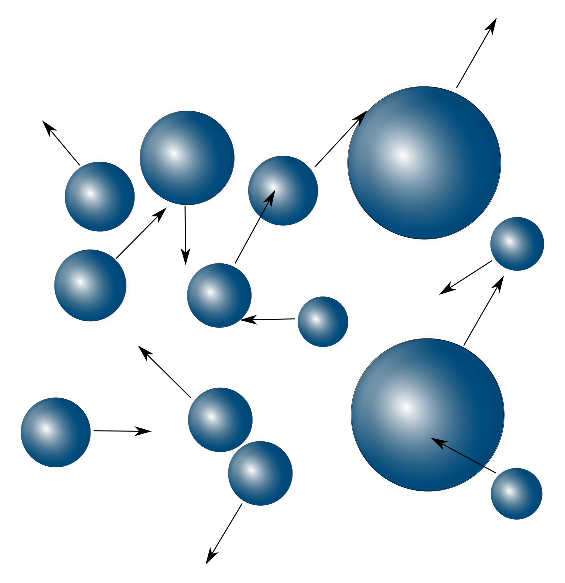
\includegraphics[width=6cm]{images/particle_system}
\caption{Das Modell des Partikelsystems, die Pfeile deuten die auf die Partikel wirkenden Kräfte an}
\end{figure}

Will man das gegebene Partikelsystem einen diskreten Zeitschritt weiterbewegen,
muss man für jedes Partikel die Kraft berechnen, die seine Beschleunigung
verursacht:

\begin{equation}
\begin{split}
F & = m \cdot a \\
  & = m \cdot \frac{\partial \vec{u}}{\partial t}
\end{split}
\end{equation}

Die Kraft, die auf alle Partikel gleich wirkt, ist die Schwerkraft:

\begin{equation}
\label{navier_stokes_f_g}
F_g = m \cdot g
\end{equation}

mit $g \cong 9.81 \frac{m}{s^2}$.

Der Druck stellt eine weitere Kraft dar. Innerhalb des Fluids gibt es Regionen
mit einer hohen Anzahl von verdichteten Partikeln (um in unserem Modell zu
bleiben) und solche mit wenigen Partikeln. Eine hohe Anzahl Partikel pro
Raumeinheit entspricht hohem Druck, wenige Partikel pro Raumeinheit entsprechen
niedrigem Druck. Hoher Druck entsteht z.B., wenn Wasser aus einer Quelle strömt
oder ein Fluid an ein Hindernis stößt.

Die Kraft, die durch den Druck ausgeübt wird, wirkt
\PimiddyQuotes{ausgleichend}, zeigt also in Regionen hohen Drucks hin zu
Regionen niedrigeren Drucks. Mathematisch gesehen ist sie proportional zum
negativen Gradient des Drucks (siehe \autoref{navier_stokes_particle_system_wall_collision}) und zum Volumen des Partikels:

\begin{equation}
\label{navier_stokes_f_p}
F_p = -\PimiddyGrad p \cdot V
\end{equation}

\begin{figure}[ht]
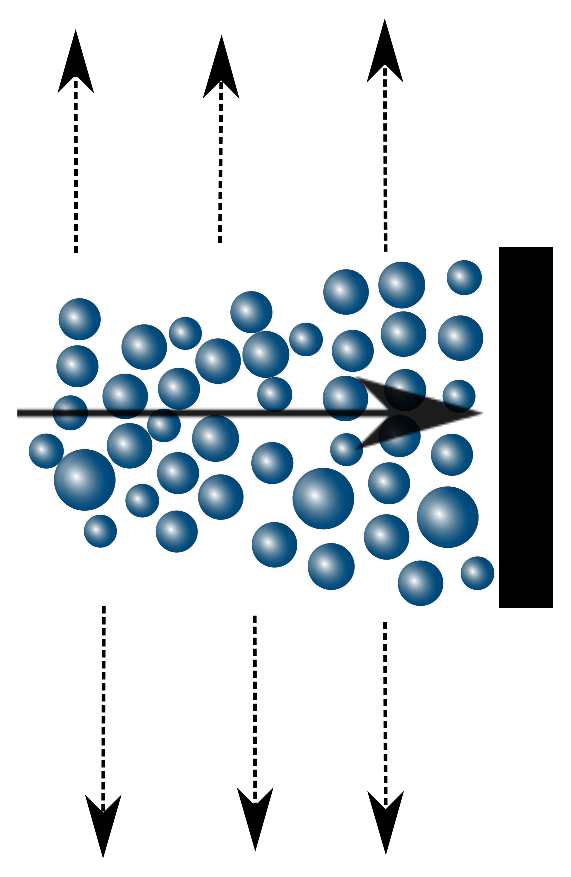
\includegraphics[width=6cm]{images/particle_system_wall_collision}
\caption{Partikelsystem, was auf ein Hindernis prallt. Der durchgezogene Pfeil deutet die Flussrichtung an, die gestrichelten Pfeile den negativen Gradienten des Drucks. Die Partikel erfahren also eine Kraft nach außen.}
\label{navier_stokes_particle_system_wall_collision}
\end{figure}

Die Viskosität des Fluids hat ebenfalls Einfluss auf die Partikel. Bei einem
viskosen Fluid wird jeder Deformation ein Widerstand entgegengesetzt. Die Kraft,
die durch die Viskosität ausgeübt wird, hat den Effekt,
Geschwindigkeitsunterschiede innerhalb des Fluids auszugleichen. Sie ist daher
proportional zum Volumen des Partikels und zum Laplace der Geschwindigkeit:

\begin{equation}
\label{navier_stokes_f_v}
F_v = \mu \cdot \PimiddyLaplace \vec{u} \cdot V
\end{equation}

Die Konstante $\mu$ stellt die \PimiddyBegriff{dynamische Viskosität} des Fluids
dar. Sie steht zur \PimiddyBegriff{kinematischen Viskosität} $\nu$ im
Verhältnis: $\nu = \mu/\rho$, wobei $\rho$ die Dichte des Fluids ist.

Mit den Gleichungen \ref{navier_stokes_f_g}, \ref{navier_stokes_f_p} und
\ref{navier_stokes_f_v} erhalten wir insgesamt:

\begin{equation}
m \cdot \frac{\partial \vec{u}}{\partial t} = m \cdot \vec{g} + -\PimiddyGrad p \cdot V + \nu \cdot \PimiddyLaplace \vec{u} \cdot V
\end{equation}

Wir wollen nun den Limes über die Masse bilden und so die Partikel beliebig
klein werden lassen. Vorher teilen wir allerdings die Gleichung noch durch das
Volumen $V$ (sonst ergibt der Limes nur $0=0$). Dies vereinfacht die Gleichung
außerdem etwas, da $m/V = \rho$ die Dichte des Fluids angibt:

\begin{equation}
\rho \cdot \frac{\partial \vec{u}}{\partial t} = \rho \cdot \vec{g} + -\PimiddyGrad p + \nu \cdot \PimiddyLaplace \vec{u} \cdot V
\end{equation}

Teilt man die Gleichung jetzt durch die Dichte $\rho$ und setzt $\nu =
\mu/\rho$, erhält man beinahe die Impulsgleichung:

\begin{equation}
\label{navier_stokes_pre_impulse_equation}
\frac{
	\partial
	\vec{u}
}
{
	\partial t
} +
\frac{
	1
}
{
	\rho
}
\PimiddyGrad p =
\vec{g} +
\nu
\PimiddyLaplace
\vec{u}
\end{equation}

Was bisher außer acht gelassen wurde, ist die \PimiddyBegriff{Konvektion}. Die
Ableitung der Geschwindigkeit $\vec{u}$ nach der Zeit zu bilden lässt den Ort
des Partikels fest. Das Partikel bewegt sich aber mit dem Strömungsfeld mit.
Daher benutzen wir die \PimiddyBegriff{substantielle Ableitung} statt der
gewöhnlichen Ableitung:

\begin{equation}
\frac{D\vec{u}}{Dt} = \frac{\partial \vec{u}}{\partial t} + \vec{u} \cdot \PimiddyDiv \vec{u}
\end{equation}

Setzen wir dies für die Ableitung nach der Zeit in \autoref{navier_stokes_pre_impulse_equation} ein, erhalten wir
die Impulsgleichung.

\subsection{Die Unkomprimierbarkeitsbedingung}

Um die Unkomprimierbarkeitsbedingung zu motivieren, sei ein beliebiges Volumen
$\Omega \subset \PimiddyReell^3$ gegeben, z.B. ein Würfel im Raum. Seine
Oberfläche sei $\partial \Omega$.

Die Änderung des Würfelvolumens über die Zeit kann berechnet werden, indem man
über die Normalenkomponente entlang seiner Oberfläche integriert \cite{Chorin1980}. Bildlich
gesprochen summiert man auf diese Weise eingehende und ausgehende Strömungen an
den Würfelseitenflächen:

\begin{equation}
\frac{
	\partial \PimiddyFormelText{Volumen}(\Omega)
}
{
	\partial t
}
=
\iint_{\partial \Omega} \vec{u} \cdot n
\end{equation}

Damit die Flüssigkeit unkomprimierbar ist, sollte dieses Integral verschwinden:

\begin{equation}
\iint_{\partial \Omega} \vec{u} \cdot n = 0
\end{equation}

Mit Hilfe des Divergenzsatzes können wir dieses Integral in ein Volumenintegral
umformen:

\begin{equation}
\iiint_\Omega \PimiddyDiv \vec{u} = 0
\end{equation}

Da $\Omega$ beliebig gewählt war, folgt $\PimiddyDiv \vec{u} = 0$.
